%
% Exemplo genérico de uso da classe destufba.cls
%
% Se você não tem familiaridade com o LaTeX, este arquivo dá algumas orientações.
% Para um aproveitamento melhor, sugere-se usar o livro LaTeX - A Document Preparation System,
% de Leslie Lamport. Na Internet estão disponíveis também alguns milhares de tutorias.
% O Departamento de Estatística oferece semestralmente um curso gratuito, fique atento.
%
% O símbolo % é um comentário de linha, então tudo que aparecer depois dele não é considerado
% no texto final. Você pode limpar todos os comentários deste arquivo, depois que colocar os
% dados corretos, sem prejuízo do texto final.
%

\documentclass[espec,ppgcdbd]{destufba}
% Para usar o modelo, deve-se informar o curso e o tipo de documento e o tipo de documento que deve ser produzido.
% Cursos:
%   * código do curso   -- Usar o código do curso, usar a sigla do programa
%                         quando se tratar de pós-graduação stricto sensu (ppgest
%                         para o Programa de Pós-graduação em Matemática (Área de 				 
%                         concentração - Estatística),por exemplo; 
%                         para especialização, definir os campos
%                         apropriadamente com o comando \course{nome-do-curso}
%                         (sem o termo ``Especialização'') e \campus{nome-do-campus}.
%   
% Tipos de Documento:
%   * tcc               -- Trabalhos de Conclusão de Curso
%   * espec             -- Monografias de Especialização
%   * mestrado          -- Dissertações de Mestrado (acadêmico)
% 
% Outras Opções:
%   * english    -- para textos em inglês
%   * openright  -- força início de capítulos em páginas ímpares (padrão da biblioteca)
%   * oneside    -- desliga frente-e-verso
%   * final      -- versão final do texto

% Programas de pós-graduação com mais de uma área de concentração devem declarar explicitamente
% a área de concentração da dissertação, por meio do comando
%\renewcommand{\areacourse}{Sanidade Animal}

\usepackage[T1]{fontenc}        % pacote para conj. de caracteres correto
%\usepackage[latin1]{inputenc}   % pacote para acentuação
\usepackage{graphicx}           % pacote para importar figuras
\usepackage{times}              % pacote para usar fonte Adobe Times
\usepackage{mathptmx}           % pacote usar fonte Adobe Times nas fórmulas
\usepackage{makecell}
\usepackage{pdfpages}

\usepackage[alf,abnt-emphasize=bf]{abntex2cite}
\usepackage[utf8]{inputenc}    % pacote para usar citações abnt

%%%%%%%%%%%%%%%%%%%%%%%%%%%%%%%%%%%%%%%%%%%%%%%%%%%%%%%%%%%%%%%%%%%%%%%%%%%%%%%
%
% Titulo e autor do trabalho.
%
%%%%%%%%%%%%%%%%%%%%%%%%%%%%%%%%%%%%%%%%%%%%%%%%%%%%%%%%%%%%%%%%%%%%%%%%%%%%%%%

\title{Uso de aprendizado de máquina para avaliar a influência das comorbidades no risco de óbito por COVID-19}

\author{Feitosa}{Taian Fonseca}

%%%%%%%%%%%%%%%%%%%%%%%%%%%%%%%%%%%%%%%%%%%%%%%%%%%%%%%%%%%%%%%%%%%%%%%%%%%%%%%
%
% Orientação (orientador é obrigatório; co-orientador é opcional)
%
%%%%%%%%%%%%%%%%%%%%%%%%%%%%%%%%%%%%%%%%%%%%%%%%%%%%%%%%%%%%%%%%%%%%%%%%%%%%%%%

\advisor[Prof.~Dr.]{Silva}{Allan Robert da}
%\coadvisor[Prof.~Dr.]{Rebouças}{Luciano Oliveira}

% Se o seu orientador ou co-orientador for mulher, acerte o nome:
%\renewcommand{\advisorname}{Orientadora}
%\renewcommand{\coadvisorname}{Co-orientadora}

%%%%%%%%%%%%%%%%%%%%%%%%%%%%%%%%%%%%%%%%%%%%%%%%%%%%%%%%%%%%%%%%%%%%%%%%%%%%%%%
%
% Definições para registro na biblioteca e banca de apresentação do trabalho
%
%%%%%%%%%%%%%%%%%%%%%%%%%%%%%%%%%%%%%%%%%%%%%%%%%%%%%%%%%%%%%%%%%%%%%%%%%%%%%%%

\cutter{---}                                                        % número de catalogação da biblioteca, na
%                                               versão final do trabalho;
%                                               deixar em branco antes de produzir a versão %                                               final.

\banca[Prof.~Dr.]{Henrique Gama Dore de Araújo}{Luiz}            % membro da banca de defesa (orientador não entra)
\inst{Universidade Federal de Sergipe}                            % instituição do membro da banca

\banca[Prof.~Dr.]{Jorge Canas Rodrigues}{Paulo}       % membro da banca de defesa
\inst{Universidade Federal da Bahia}                            % instituição do membro da banca

% \banca[Dr.]{definir}{A}                        % membro da banca de defesa
% \inst{Universidade Federal da Bahia}                                      % instituição do membro da banca

\defesa{02}{dezembro}{2022}                       % data da defesa - dia, mês e ano

%%%%%%%%%%%%%%%%%%%%%%%%%%%%%%%%%%%%%%%%%%%%%%%%%%%%%%%%%%%%%%%%%%%%%%%%%%%%%%%%

% A data deve ser a da defesa ou a da geração do documento, o que vier primeiro;
% se nao especificada, são gerados mês e ano correntes. Use somente se for gerar
% novamente o documento após a defesa.
%\date{maio}{2001}

% O local de realização do trabalho deve ser especificado
% com o comando \location.
\location{Salvador}{BA}

%
% Palavras-chave para o resumo (na língua do documento)
%
% Iniciar todas com a primeira legra maiúscula e as demais letras minúsculas,
% exceto no caso de abreviaturas.
%
\keyword{COVID-19}
\keyword{SRAG}
\keyword{Comorbidades}
\keyword{Aprendizado de máquina}
\keyword{OPENDATASUS}

\sloppy % para o texto não ficar esquisito quando se usar elementos muito compridos que não podem ser separados.

% ---------------------------------------------------------------------------- %
\graphicspath{{./figuras/}}             % caminho das figuras (recomendável)
% ---------------------------------------------------------------------------- %

%
% Início do documento
%

\begin{document}

%
% Produção das folhas de rosto, da ficha catalográfica do documento e da folha de aprovação.
% Se todos os dados acima foram preenchidos corretamente, as folhas de rosto devem sair no formato correto.
%

    \maketitle

%
% Dedicatoria (opcional)
%

    \begin{dedicatoria}
        Dedico este trabalho a Ellen, o meu amor mais lindo mundo <3
    \end{dedicatoria}

%
% Agradecimentos (opcional)
%
% Se você tiver muito a agradecer, pode usar um arquivo à parte e incluí-lo
% no texto, por meio do comando \input{meus-agradecimenos}. O compilador
% LaTeX buscará o arquivo meus-agradecimentos.tex e incluirá o texto do mesmo
% neste local. Isso ajuda a tornar o arquivo principal do trabalho (este)
% mais limpo, claro e conciso.
%

    \chapter*{Agradecimento}
    Agradeço à UFBA ....

%
% Epígrafe (opcional)
%
    \begin{epigrafe}
        ``Errar e aprender com os erros é humano. Aprender errando milhares de vezes por segundo, é inteligência artificial.''\\
        --- Taian Feitosa
    \end{epigrafe}

%
% Resumo na língua do documento (obrigatório). Deve ser escrito em um único parágrafo:
%

    \begin{abstract}
        \emph{
            O objetivo deste trabalho é usar algoritmos de aprendizado de máquina para avaliar a influência de comorbidades no risco de óbito por COVID-19. Os dados de pacientes com Síndrome Respiratória Aguda Grave (SRAG) foram extraídos do OPENDATASUS, portal do Ministério da Saúde do Brasil, no dia 12 de outubro de 2022. Sete algoritmos foram utilizados para avaliar os dados. Alguns deles, como o algoritmo de Regressão Logística, geram coeficientes que possuem interpretação matemática, que foram utilizados para avaliar e comparar o grau de risco de morte em pacientes com COVID-19, com e sem comorbidades.
        }
    \end{abstract}

%
% Resumo na outra língua - se o texto for em Português, o abstract é em Inglês e vice-versa -
% como parâmetros devem ser passadas as palavras-chave na outra língua, separadas por vírgulas:
%

    \begin{englishabstract}{COVID-19, SARS, Comorbidities, Machine learning, OPENDATASUS}
        \emph{
            The objective of this work is to use machine learning algorithms to evaluate the influence of comorbidities on the risk of death from COVID-19. The data of patients with Severe Acute Respiratory Syndrome (SARS) were extracted from OPENDATASUS, the portal of the Brazilian Ministry of Health, on October 12, 2022. Seven algorithms were used to evaluate the data. Some of them, such as the Logistic Regression algorithm, generate coefficients that have mathematical interpretation, which were used to assess and compare the degree of risk of death in patients with COVID-19, with and without comorbidities.
        }
    \end{englishabstract}

%
% Lista de figuras
%
% Todas as figuras declaradas no texto dentro de um ambiente figure serão numeradas apropriadamente e
% colocadas automaticamente nesta lista, com o número de página onde aparecem correto:
%
    % \listoffigures

%
% Lista de tabelas
%
% Todas as tabelas declaradas no texto dentro de um ambiente table serão numeradas apropriadamente e
% colocadas automaticamente nesta lista, com o número de página onde aparecem correto:
%

    \listoftables

% Listas de definições e teoremas, para quem usar o pacote formais, para trabalhos que possuam definições formais e teoremas

%\listofdefinitions
%\listoftheorems

%
% Lista de abreviaturas e siglas
%
% O parâmetro deve ser a abreviatura mais longa. Essa lista é opcional, mas é muito conveniente.
% Só não abuse. use somente siglas consagradas. Se quiser economizar na escrita, use o comando
% \newcommand{\MT}{Máquina de Turing} e use \MT sempre que quiser que o termo apareça completo.
% Isso torna a leitura do texto mais fluente.
    \begin{listofabbrv}{destufba}
        % \item[ABNT]     Associação Brasileira de Normas Técnicas
        % \item[ACM]      Association for Computing Machinery
        % \item[IEEE]     Institute of Electrical and Electronics Engineers
        % \item[IP]       Internet Protocol
        % \item[RTP]      Real-Time Protocol
        % \item[RSSF]     Rede de Sensores sem Fio
        % \item[SIMD]     Single Instruction Multiple Data
        \item[COVID] Coronavirus disease (doença do coronavírus)
        \item[FM] Factorization Machines
        \item[LASSO] Least Absolute Shrinkage and Selection Operator
        \item[MLP] Multilayer Perceptron
        \item[SRAG] Síndrome Respiratória Aguda Grave
        \item[SVM] Support Vector Machines
        \item[UFBA] Universidade Federal da Bahia
        % \item[UFRGS]    Universidade Federal do Rio Grande do Sul
    \end{listofabbrv}

% Lista de símbolos
    \begin{listofsymbols}{$\alpha\beta\pi\omega$}
%        \item[$\sum{\frac{a}{b}}$] Somatório do produtório
%        \item[$\alpha\beta\pi\omega$] Fator de inconstância do resultado
        \item[$\beta$] Coeficiente da regressão logística
        \item[$\prod$] Produtório
    \end{listofsymbols}

%%%%%%%%%%%%%%%%%%%%%%%%%%%%%%%%%%%%%%%%%%%%%%%%%%%%%%%%%%%%%%%%%%%%%%%%%%%%
%
% Sumário - elemento obrigatório do trabalho - gerado automaticamente com
%           o comando abaixo.
%
%%%%%%%%%%%%%%%%%%%%%%%%%%%%%%%%%%%%%%%%%%%%%%%%%%%%%%%%%%%%%%%%%%%%%%%%%%%%

    \tableofcontents

%%%%%%%%%%%%%%%%%%%%%%%%%%%%%%%%%%%%%%%%%%%%%%%%%%%%%%%%%%%%%%%%%%%%%%%%%%%%
%
% Aqui comeca o texto propriamente dito. O texto pode ser todo escrito neste
% mesmo arquivo, mas pode-se separar o texto em diversos arquivos, que podem
% ser incluídos com o comando \input{nome-do-arquivo} (inclui o arquivo com
% nome nome-do-arquivo.tex), que deve estar no mesmo diretório do texto
% principal. Se estiver em outro diretório, pode ser incluído também, usando
% \input{Textos/nome-do-arquivo}. Dessa forma, o arquivo será buscado no
% subdiretório Textos; se quiser usar caminhos na árvore de diretórios, use
% \input{../Textos/nome-do-arquivo}, que procura o arquivo que está no diretório
% Textos, um nível acima na estrutura.
%
%%%%%%%%%%%%%%%%%%%%%%%%%%%%%%%%%%%%%%%%%%%%%%%%%%%%%%%%%%%%%%%%%%%%%%%%%%%%

% E aqui vai a parte principal:


    \chapter{Metodologia}
\label{ch:metodologia}

Para alcançar o objetivo deste trabalho, que consiste em analisar o risco de morte em pacientes hospitalizados com COVID-19, conforme as comorbidades, utilizou-se alguns algoritmos de aprendizado de máquina para tentar predizer se o paciente com COVID-19 sobreviverá ou não a esta doença.
Os dados dos hospitalizados foram obtidos no portal OPENDATASUS~\cite{opendatasus2020,opendatasus20212022} no dia 12 de outubro.

As comorbidades catalogadas pelo OPENDATASUS e utilizadas neste trabalho foram:

\begin{itemize}
    \item Doença Cardiovascular Crônica
    \item Doença Hematológica Crônica
    \item Síndrome de Down
    \item Doença Hepática Crônica
    \item Asma
    \item Diabetes mellitus
    \item Doença Neurológica Crônica
    \item Outra Pneumatopatia Crônica
    \item Imunodeficiência ou Imunodepressão
    \item Doença Renal Crônica
    \item Obesidade
\end{itemize}

Os dados disponibilizados foram filtrados para apenas os casos confirmados como COVID-19 e com evolução desconhecida foram descartados.
Como alguns algoritmos são especialmente sensíveis quando a classe de avaliação é desbalanceada, e como a base possui mais curados do que óbitos, foi realizado um \textit{undersampling}, foram sorteados aleatoriamente uma quantidade de curados dentre a base de entrada para que os dados de treino tenha uma quantidade semelhante de dados entre as classes.

Os algoritmos foram treinados com Apache Spark, ``um motor multilinguagem para executar engenharia de dados, ciências de dados e aprendizado de máquina em máquinas de nó único ou `clusters'\,''~\cite{apachespark}.
O Spark permite realizar validação cruzada para treinar o modelo e utilizar uma matriz de parâmetros para selecionar automaticamente o melhor conjunto de parâmetros, através do avaliador selecionado~\cite{apachesparkcv}.
Dentre os algoritmos implementados no Spark~\cite{apachesparkml}, este trabalho testou os seguintes:

\begin{itemize}
    \item Regressão logística
    \item Floresta aleatória
    \item \textit{Gradient boosting} em árvore
    \item Perceptron multicamadas
    \item Máquina de vetores de suporte
    \item \textit{Naïve Bayes}
    \item Máquinas de Fatoração
\end{itemize}

A regressão logística calcula valores que possuem interpretação matemática para modelar a probabilidade de um evento ocorrer, conforme a presença de outro.
Por isso, esses valores serão utilizados para ranquear as comorbidades com maior influência no risco de morte.
As matrizes de parâmetros serão abordadas em~\ref{ch:modelos}.
O código utilizado nesse trabalho, feito na linguagem Scala, está disponível no repositório do GitHub \href{https://github.com/taianf/ECD-TCC-Dados}~\cite{githubtcc}.

    \chapter{Fundamentos}
\label{ch:fundamentos}

O aprendizado de máquinas (Machine Learning, em inglês) é um campo de estudo dedicado à compreensão e construção de métodos que `aprendem', ou seja, métodos que usam os dados para melhorar o desempenho em algum conjunto de tarefas~\cite{mitcheltom}.
Os algoritmos de aprendizado de máquinas constroem um modelo baseado em dados de amostra, conhecidos como dados de treino, a fim de fazer previsões ou tomar decisões sem serem explicitamente programados para isso~\cite{simonphill}.

Os métodos de aprendizado de máquina são classificados basicamente em três tipos~\cite{russellstuart}:

\begin{itemize}
    \item Aprendizado supervisionado:
    \subitem Exemplos de entradas e saídas pré-classificadas são apresentados ao computador.
    O objetivo é aprender uma regra geral que mapeia entradas para saídas.

    \item Aprendizado não supervisionado:
    \subitem Nenhum tipo de classificação é dado ao algoritmo de aprendizado, deixando-o sozinho para encontrar relacionamentos nas entradas fornecidas.
    O aprendizado não supervisionado pode ser um objetivo em si, descobrir novos padrões nos dados, ou um meio para um fim.

    \item Aprendizado por reforço:
    \subitem Um programa de computador interage com um ambiente dinâmico, no qual o programa deve realizar um determinado objetivo (por exemplo, dirigir um veículo).
    O feedback sobre recompensas e punições é fornecido ao programa à medida que ele navega no espaço do problema.
    Outro exemplo de aprendizado por reforço é aprender a jogar um determinado jogo apenas jogando contra um oponente.
\end{itemize}

Existem algumas técnicas para juntar vários modelos em um só, como \textit{ensemble} e \textit{boosting}.

Os métodos \textit{ensemble} utilizam múltiplos algoritmos de aprendizado para obter um melhor desempenho preditivo do que o que poderia ser obtido apenas com qualquer um dos algoritmos de aprendizado constituintes.
Ao contrário de um \textit{ensemble} estatístico em mecânica estatística, que é geralmente infinito, um \textit{ensemble} de aprendizado de máquinas consiste apenas num conjunto finito concreto de modelos alternativos, mas tipicamente permite que exista uma estrutura muito mais flexível entre essas alternativas~\cite{ensemble}.

\textit{Boosting} é um método de \textit{ensemble} que combina um conjunto de modelos fracos num modelo forte para minimizar erros de treino.
No \textit{boosting}, uma amostra aleatória de dados é selecionada, treinada com um modelo e depois treinada sequencialmente, isto é, cada modelo tenta compensar as fraquezas do seu predecessor.
Com cada iteração as regras fracas de cada classificador individual são combinadas para formar uma regra de previsão forte~\cite{boosting}.

Os dados deste trabalho já estão pré-classificados, portanto foram utilizados alguns modelos de aprendizado supervisionado.
Os modelos neste trabalho e citados no capítulo~\ref{ch:metodologia} foram escolhidos pois já tem algoritmos de treinamento presentes no Apache Spark.
Para mais detalhes sobre a implementação dos modelos no Apache Spark é possível conferir a documentação oficial~\cite{apachesparkml}.

\section{Regressão Logística}
\label{sec:fun:lr}

A regressão logística é uma técnica estatística que visa produzir, a partir de um conjunto de observações, um modelo que permita a previsão de valores tomados por uma variável categórica, muitas vezes binária, a partir de uma série de variáveis explicativas contínuas ou binárias.
É um caso especial de modelos Lineares Generalizados que prevê a probabilidade dos resultados~\cite{glmarticle}.

A regressão logística tem a vantagem de ter uma interpretação prática para os coeficientes, onde eles representam a probabilidade de um evento ocorrer em função de outros fatores.
Essa interpretação pode ajudar a descobrir quais variáveis são relevantes para o modelo e quais não são.
Por ser um modelo simples de treinar e possuir coeficientes interpretáveis, é frequentemente utilizado como base para comparação da eficiência de outros modelos treinados.

A interpretação dos coeficientes se dá pela equação~\ref{eq:prob-rl}.
Coeficientes $\beta$ positivos indicam que a probabilidade da classe avaliada aumenta quando o fator é positivo enquanto coeficientes $\beta$ negativos indicam que a probabilidade diminui.

\begin{equation}
    \label{eq:prob-rl}
    p_i = e^{\beta_i}
\end{equation}

Por exemplo, um coeficiente $\beta_i = 0,1$ gera um $p_i = 1,105171$, significando que quando o fator $i$ está presente, a probabilidade da classe alvo ser positiva é aproximadamente 10,5171\% maior se comparado a quando o fator $i$ está ausente.

O intercepto $\beta_0$ representa a probabilidade da classe alvo ser positiva quando todos os coeficientes são 0 e seu cálculo se dá pela equação~\ref{eq:int-rl}.

\begin{equation}
    \label{eq:int-rl}
    p = \frac{e^{\beta_0}}{(1 + e^{\beta_0}) }
\end{equation}

\section{Floresta Aleatória}
\label{sec:fun:rf}

Florestas aleatórias ou florestas de decisão aleatória é um método de aprendizado \textit{ensemble} para classificação, regressão e outras tarefas que opera construindo várias árvores de decisão em tempo de treinamento~\cite{hotimkam}.
O aprendizado de árvore de decisão é uma abordagem de aprendizado supervisionado usada em estatística, mineração de dados e aprendizado de máquina~\cite{decisiontree}.
Uma árvore é construída dividindo o conjunto fonte, que constitui o nó raiz da árvore, em subconjuntos – que constituem os filhos sucessores.
Esse processo é repetido em cada subconjunto.
A recursão é concluída quando o subconjunto em um nó tem todos os mesmos valores que a variável de destino, ou quando a divisão não agrega mais valor às previsões.

Para tarefas de classificação, a saída da floresta aleatória é a classe selecionada pela maioria das árvores.
Para tarefas de regressão, a previsão média das árvores individuais é retornada.
Florestas de decisão aleatórias diminuem a chance de \textit{overfitting} das árvores de decisão ao seu conjunto de treinamento.
As florestas aleatórias geralmente superam as árvores de decisão, mas sua precisão é menor do que o \textit{Gradient boosting} em árvore, visto na seção~\ref{sec:fun:gbt}.

\section{\textit{Gradient boosting} em árvore}
\label{sec:fun:gbt}

O \textit{Gradient boosting} é uma técnica de aprendizado de máquina usada em tarefas de regressão e classificação, entre outras.
Fornece um modelo de previsão sob a forma de um conjunto de modelos de previsão fracos, que são tipicamente árvores de decisão~\cite{gbta1,elementsofstatisticallearning}.
Quando uma árvore de decisão é o modelo fraco, o algoritmo resultante é chamado de árvores de gradiente e normalmente tem um desempenho superior ao da floresta aleatória.


\section{Perceptron multicamadas}
\label{sec:fun:mlp}

Um perceptron multicamadas (Multilayer perceptron ou MLP em inglês) é uma classe de rede neural artificial feedforward totalmente ligada.
O termo MLP é utilizado ambiguamente, por vezes de forma solta para significar qualquer rede neural artificial de alimentação, por vezes estritamente para se referir a redes compostas de múltiplas camadas de perceptrons.
Os perceptrons multicamadas são por vezes referidos coloquialmente como redes neurais ``baunilha'', especialmente quando têm uma única camada oculta~\cite{elementsofstatisticallearning}.

Um MLP consiste em pelo menos três camadas de nós: uma camada de entrada, uma camada oculta e uma camada de saída.
Com excepção dos nós de entrada, cada nó é um neurônio que utiliza uma função de ativação não linear.
O MLP utiliza uma técnica de aprendizado supervisionado chamada \textit{backpropagation} para treino.
As suas múltiplas camadas e ativação não linear distinguem o MLP de um perceptron linear e pode distinguir os dados que não são separáveis linearmente~\cite{perceptrons}.

\section{Máquina de vetores de suporte}
\label{sec:fun:lsvc}

No aprendizado de máquinas, as máquinas de vetores de suporte (Support Vector Machines, SVMs em inglês) são modelos de aprendizado supervisionados com algoritmos de aprendizado associados que analisam dados para classificação e regressão.
Dado um conjunto de exemplos de formação, cada um marcado como pertencendo a uma de duas categorias, um algoritmo de SVM constrói um modelo que atribui novos exemplos a uma ou outra categoria, tornando-o um classificador linear binário não probabilístico, embora existam métodos para utilizar SVM num cenário de classificação probabilístico.

A SVM mapeia exemplos de formação para pontos no espaço de modo a maximizar a largura do intervalo entre as duas categorias.
Novos exemplos são então mapeados para esse mesmo espaço e prevê-se que pertençam a uma categoria com base em que lado do intervalo caem.
Além de realizar a classificação linear, as SVMs podem realizar eficientemente uma classificação não linear usando o que é chamado de \textit{kernel trick}, mapeando implicitamente suas entradas em espaços de características de dimensões mais altas~\cite{svms}.

\section{Classificadores \textit{Naïve Bayes}}
\label{sec:fun:nb}

Em estatística, os classificadores \textit{Naïve Bayes} são uma família de simples ``classificadores probabilísticos'' baseados na aplicação do teorema Bayes com fortes suposições de independência entre as características.
Eles estão entre os modelos de rede Bayes mais simples, mas podem atingir altos níveis de precisão~\cite{bayes,elementsofstatisticallearning}.

Os classificadores Naive Bayes são altamente escaláveis, exigindo uma série de parâmetros lineares no número de variáveis (características/previsões) em um problema de aprendizado.
O treinamento de máxima probabilidade pode ser feito avaliando uma expressão de forma fechada, que leva tempo linear, ao invés de uma aproximação iterativa cara como a utilizada para muitos outros tipos de classificadores.


\section{Máquinas de fatoração}
\label{sec:fun:fm}

As máquinas de fatoração (Factorization Machines - FM em inglês) são capazes de estimar as interações entre as características, mesmo em problemas com grande esparsidade (muitos valores zero ou ausentes).
FM pode ser usada para regressão e o critério de otimização é o erro quadrático médio.
FM também pode ser usada para classificação binária através da função sigmóide e o critério de otimização é a perda logística~\cite{facmachineo,apachesparkml}.


    \chapter{Modelos}
\label{ch:modelos}

Para treinar os modelos com validação cruzada no Spark, uma matriz de parâmetros foi fornecida para cada treino.
Isso faz o Spark treinar uma quantidade de modelos dada pela equação~\ref{eq:qtd-modelos}, onde $k$ é o número de \textit{folds} na validação cruzada e $p_{i}$ é o número de parâmetros a treinar no i-ésimo hiperparâmetro.
Isso implica que de testar muitos parâmetros eleva o tempo de treino.
Neste trabalho foi usado $k = 3$ para todos os treinos e veremos em cada seção os parâmetros para cada modelo treinado.

\begin{equation}
    \label{eq:qtd-modelos}
    k \times \prod_{i=0}^{n} p_i
\end{equation}

\section{Regressão Logística}
\label{sec:lr}

Para treinar o modelo de regressão logística, a matriz de parâmetros na tabela~\ref{tab:param-lr} foi utilizada.
Pela equação~\ref{eq:qtd-modelos}, foram treinados 135 ($3 \times 3 \times 5 \times 3$) modelos de regressão logística.
Os parâmetros selecionados estão presentes na tabela~\ref{tab:param-final-lr}.

\begin{table}[h]
    \centering
    \begin{tabular}{|c|c|c|}
        \hline
        Parâmetro                & Valores                   \\ \hline
        \textit{regParam}        & 0.01, 0.02, 0.1           \\
        \textit{elasticNetParam} & 0.0, 0.25, 0.5, 0.75, 1.0 \\
        \textit{maxIter}         & 1, 2, 3                   \\ \hline
    \end{tabular}
    \caption{Parâmetros para treino da regressão logística}
    \label{tab:param-lr}
\end{table}

\begin{table}[h]
    \centering
    \begin{tabular}{|c|c|c|}
        \hline
        Parâmetro                & Valor \\ \hline
        \textit{regParam}        & 0.1   \\
        \textit{elasticNetParam} & 0.0   \\
        \textit{maxIter}         & 2     \\ \hline
    \end{tabular}
    \caption{Parâmetros selecionados na validação cruzada da regressão logística}
    \label{tab:param-final-lr}
\end{table}

\textit{regParam}: é o parâmetro de regularização.
A regularização serve para prevenir \textit{overfitting}, penalizando modelos com valores de coeficiente muito altos.
Coeficientes muito altos podem ocorrer quando há algum parâmetro raro que força uma correlação muito alta com a variável a ser estimada.

\textit{elasticNetParam}: é o parâmetro de proporção da \textit{Elastic-net}.
Este parâmetro fica entres os limites 0 e 1.
Quando o valor é 0 a penalidade aplicada é do tipo L2~(\textit{Ridge}) e quando o valor é 1 a penalidade aplicada é do tipo L1~(\textit{LASSO}).

\textit{maxIter}: a quantidade máxima de iterações do algoritmo.

\section{Floresta Aleatória}
\label{sec:rf}

Para treinar a floresta aleatória, a matriz de parâmetros na tabela~\ref{tab:param-rf} foi utilizada.
Pela equação~\ref{eq:qtd-modelos}, foram treinados 45 ($3 \times 3 \times 5$) modelos.
Os parâmetros selecionados estão presentes na tabela~\ref{tab:param-final-rf}.

\begin{table}[h]
    \centering
    \begin{tabular}{|c|c|c|}
        \hline
        Parâmetro         & Valores           \\ \hline
        \textit{numTrees} & 10, 20, 30        \\
        \textit{maxDepth} & 5, 10, 15, 25, 30 \\ \hline
    \end{tabular}
    \caption{Parâmetros para treino da floresta aleatória}
    \label{tab:param-rf}
\end{table}

\begin{table}[h]
    \centering
    \begin{tabular}{|c|c|c|}
        \hline
        Parâmetro         & Valores \\ \hline
        \textit{numTrees} & 20      \\
        \textit{maxDepth} & 15      \\ \hline
    \end{tabular}
    \caption{Parâmetros selecionados na validação cruzada da floresta aleatória}
    \label{tab:param-final-rf}
\end{table}

\textit{numTrees}: o número de árvores que devem compor a floresta aleatória.

\textit{maxDepth}: a profundidade máxima das árvores geradas.

\section{\textit{Gradient boosting} em árvore}
\label{sec:gbt}

Para treinar o modelo de \textit{gradient boosting} em árvore, a matriz de parâmetros na tabela~\ref{tab:param-gbt} foi utilizada.
Pela equação~\ref{eq:qtd-modelos}, foram treinados 27 ($3 \times 3 \times 3$) modelos.
Os parâmetros selecionados estão presentes na tabela~\ref{tab:param-final-gbt}.

\begin{table}[h]
    \centering
    \begin{tabular}{|c|c|c|}
        \hline
        Parâmetro         & Valores    \\ \hline
        \textit{maxIter}  & 10, 20, 30 \\
        \textit{maxDepth} & 2, 6, 10   \\ \hline
    \end{tabular}
    \caption{Parâmetros para treino do \textit{gradient boosting} em árvore}
    \label{tab:param-gbt}
\end{table}

\begin{table}[h]
    \centering
    \begin{tabular}{|c|c|c|}
        \hline
        Parâmetro         & Valores \\ \hline
        \textit{maxIter}  & 20      \\
        \textit{maxDepth} & 6       \\ \hline
    \end{tabular}
    \caption{Parâmetros selecionados na validação cruzada do \textit{gradient boosting} em árvore}
    \label{tab:param-final-gbt}
\end{table}

\textit{maxIter}: a quantidade máxima de iterações do algoritmo.

\textit{maxDepth}: a profundidade máxima das árvores geradas.

\section{Perceptron multicamadas}
\label{sec:mlp}

Para treinar o modelo de perceptron multicamadas, a matriz de parâmetros na tabela~\ref{tab:param-mlp} foi utilizada.
Pela equação~\ref{eq:qtd-modelos}, foram treinados 18 ($3 \times 6$) modelos.
Os parâmetros selecionados estão presentes na tabela~\ref{tab:param-final-mlp}.

\begin{table}[h]
    \centering
    \begin{tabular}{|c|c|c|}
        \hline
        Parâmetro       & Valores                  \\ \hline
        \textit{layers} & \makecell{(12, 5, 5, 2),\\(12, 10, 10, 2),\\(12, 20, 20, 2),\\(12, 5, 5, 5, 2),\\(12, 10, 10, 10, 2),\\(12, 20, 20, 20, 2)} \\ \hline
    \end{tabular}
    \caption{Parâmetros para treino do perceptron multicamadas}
    \label{tab:param-mlp}
\end{table}

\begin{table}[h]
    \centering
    \begin{tabular}{|c|c|c|}
        \hline
        Parâmetro       & Valores             \\ \hline
        \textit{layers} & (12, 10, 10, 10, 2) \\ \hline
    \end{tabular}
    \caption{Parâmetros selecionados na validação cruzada do perceptron multicamadas}
    \label{tab:param-final-mlp}
\end{table}

\textit{layers}: uma sequência com a quantidade de neurônios em cada camada.

\section{Máquina de vetores de suporte}
\label{sec:lsvc}

Para treinar o modelo de Máquina de vetores de suporte, a matriz de parâmetros na tabela~\ref{tab:param-lsvc} foi utilizada.
Pela equação~\ref{eq:qtd-modelos}, foram treinados 27 ($3 \times 3 \times 3$) modelos.
Os parâmetros selecionados estão presentes na tabela~\ref{tab:param-final-lsvc}.

\begin{table}[h]
    \centering
    \begin{tabular}{|c|c|c|}
        \hline
        Parâmetro         & Valores         \\ \hline
        \textit{maxIter}  & 1, 2, 3         \\
        \textit{regParam} & 0.01, 0.02, 0.1 \\ \hline
    \end{tabular}
    \caption{Parâmetros para treino da Máquina de vetores de suporte}
    \label{tab:param-lsvc}
\end{table}

\begin{table}[h]
    \centering
    \begin{tabular}{|c|c|c|}
        \hline
        Parâmetro         & Valores \\ \hline
        \textit{maxIter}  & 3       \\
        \textit{regParam} & 0.02    \\ \hline
    \end{tabular}
    \caption{Parâmetros selecionados na validação cruzada da Máquina de vetores de suporte}
    \label{tab:param-final-lsvc}
\end{table}

\textit{maxIter}: a quantidade máxima de iterações do algoritmo.

\textit{regParam}: é o parâmetro de regularização.
A regularização serve para prevenir \textit{overfitting}, penalizando modelos com valores de coeficiente muito altos.
Coeficientes muito altos podem ocorrer quando há algum parâmetro raro que força uma correlação muito alta com a variável a ser estimada.

\section{Classificadores \textit{Naïve Bayes}}
\label{sec:nb}

Para treinar o modelo de Classificadores \textit{Naïve Bayes}, não foi utilizada nenhuma matriz de parâmetros.
Portanto foram treinados apenas 3 modelos, devido ao $k$ ser igual a 3.

\section{Máquinas de fatoração}
\label{sec:fm}

Para treinar o modelo de Máquinas de fatoração a matriz de parâmetros na tabela~\ref{tab:param-fm} foi utilizada.
Pela equação~\ref{eq:qtd-modelos}, foram treinados 135 ($3 \times 3 \times 3 \times 5$) modelos.
Os parâmetros selecionados estão presentes na tabela~\ref{tab:param-final-fm}.

\begin{table}[h]
    \centering
    \begin{tabular}{|c|c|c|}
        \hline
        Parâmetro         & Valores                       \\ \hline
        \textit{maxIter}  & 1, 5, 10                      \\
        \textit{regParam} & 0.01, 0.02, 0.1               \\
        \textit{stepSize} & 0.001, 0.005, 0.01, 0.05, 0.1 \\ \hline
    \end{tabular}
    \caption{Parâmetros para treino das Máquinas de fatoração}
    \label{tab:param-fm}
\end{table}

\begin{table}[h]
    \centering
    \begin{tabular}{|c|c|c|}
        \hline
        Parâmetro         & Valores \\ \hline
        \textit{maxIter}  & 10      \\
        \textit{regParam} & 0.02    \\
        \textit{stepSize} & 0.1     \\ \hline
    \end{tabular}
    \caption{Parâmetros selecionados na validação cruzada das Máquinas de fatoração}
    \label{tab:param-final-fm}
\end{table}

\textit{maxIter}: a quantidade máxima de iterações do algoritmo.

\textit{regParam}: é o parâmetro de regularização.
A regularização serve para prevenir \textit{overfitting}, penalizando modelos com valores de coeficiente muito altos.
Coeficientes muito altos podem ocorrer quando há algum parâmetro raro que força uma correlação muito alta com a variável a ser estimada.

\textit{stepSize}: o tamanho do incremento a cada iteração.


    \chapter{Análises}
\label{ch:analises}

Os dados disponíveis no OPENDATASUS possuem 3.443.459 entradas e totalizam 1,87GB em arquivos no formato csv (\textit{comma separated values}).
Filtrando os dados de interesse totalizam 990.466 entradas.
Estas entradas foram separadas em 8o\% para treino e validação e 20\% para teste.
Estes 80\% foram usados na validação cruzada.
A cada iteração dois terços desses 80\% foram usados para treino e um terço usado para avaliação dos modelos gerados.
O melhor modelo gerado nas iterações é avaliado com os dados separados para teste.

Para analisar os modelos de classificação gerados podemos usar algumas métricas: \textit{Accuracy}, \textit{Precision}, \textit{Recall} e \textit{F1 Score}.
Estas métricas são calculadas com base nos valores de Verdadeiros Positivos (VP), Falsos Positivos (FP), Falsos Negativos (FN) e Verdadeiros Negativos (VN).
Esse valores aparecem na Matriz de Confusão dos modelos gerados pelo Apache Spark.

\begin{table}[h]
    \centering
    \begin{tabular}{|c|c|c|}
        \hline
        Valor real \textbackslash{} Classificação do modelo & Positivo & Negativo \\ \hline
        Positivo                                            & VP       & FN       \\ \hline
        Negativo                                            & FP       & VN       \\ \hline
    \end{tabular}
    \caption{Matriz de confusão}
    \label{tab:matriz-confusao}
\end{table}

\textit{Accuracy}~(\ref{eq:accuracy}), acurácia em português, é a divisão entre todos os acertos pelo total de previsões.

\begin{equation}
    \label{eq:accuracy}
    \frac{VP + VN}{VP + VN + FP + FN}
\end{equation}

\textit{Precision}~(\ref{eq:precision}), precisão em português, é a divisão entre os Verdadeiros Positivos e todas as previsões positivas.

\begin{equation}
    \label{eq:precision}
    \frac{VP}{VP + FP}
\end{equation}

\textit{Recall}~(\ref{eq:recall}), revocação em português, é a divisão entre os Verdadeiros Positivos e todas os valores que realmente são positivos.

\begin{equation}
    \label{eq:recall}
    \frac{VP}{VP + FN}
\end{equation}

\textit{F1 Score}~(\ref{eq:f1score}), é a média harmônica entre \textit{Precision} e \textit{Recall}.

\begin{equation}
    \label{eq:f1score}
    \frac{2 * Precision * Recall}{Precision + Recall}
\end{equation}

\section{Comparativo entre modelos}
\label{sec:comparativo-entre-modelos}

Uma primeira análise a se fazer, é comparar o custo de treino de cada modelo.
Todos os modelos foram treinados na mesma máquina, cujas especificações encontram-se no apêndice~\ref{ch:maquina}.

\begin{table}[h]
    \centering
    \begin{tabular}{|l|r|r|r|}
        \hline
        Modelo                               & Tempo (s) & Quantidade & Tempo/modelo \\
        \hline
        Regressão Logística                  & 1140      & 135        & 8.4          \\
        Máquinas de fatoração                & 1317      & 135        & 9.8          \\
        Floresta Aleatória                   & 1002      & 145        & 22.3         \\
        Máquina de vetores de suporte        & 813       & 27         & 30.1         \\
        \textit{Naïve Bayes}                 & 106       & 3          & 35.3         \\
        \textit{Gradient boosting} em árvore & 2082      & 127        & 77.1         \\
        Perceptron multicamadas              & 1759      & 18         & 97.7         \\
        \hline
    \end{tabular}
    \caption{Tempo de treinamento dos modelos}
    \label{tab:modelos-tempo}
\end{table}

Modelos mais simples levam menos tempo para ser treinados pois exigem menos recursos computacionais e são preferidos quando a eficiências entre diferentes modelos forem parecidas.
Como vemos na tabela~\ref{tab:modelos-tempo} os modelos de regressão logística e máquinas de fatoração foram mais eficientes que os demais modelos, enquanto \textit{Gradient boosting} em árvore e Perceptron multicamadas tiveram um custo maior que os demais.

\subsection{\textit{Accuracy}}
\label{subsec:accuracy}

\begin{table}[h]
    \centering
    \begin{tabular}{|l|r|c|}
        \hline
        Modelo                               & Tempo/modelo & \textit{Accuracy}  \\
        \hline
        \textit{Gradient boosting} em árvore & 77.1         & 0.6788676814045260 \\
        Floresta Aleatória                   & 22.3         & 0.6787368124345655 \\
        Máquina de vetores de suporte        & 30.1         & 0.6784046065877426 \\
        Perceptron multicamadas              & 97.7         & 0.6780019328340179 \\
        Máquinas de fatoração                & 9.8          & 0.6767838447290005 \\
        Regressão Logística                  & 8.4          & 0.6764516388821776 \\
        \textit{Naïve Bayes}                 & 35.3         & 0.6735221873238302 \\
        \hline
    \end{tabular}
    \caption{\textit{Accuracy} dos modelos}
    \label{tab:modelos-accuracy}
\end{table}

Na tabela~\ref{tab:modelos-accuracy} todos os modelos tem uma \textit{Accuracy} bem próximas.
A diferença entre o melhor e o pior modelo é de 0.00534549408, ou 0.534549408\%.
Vamos analisar as outras métricas para diferenciar melhor os modelos.

\subsection{\textit{Precision}}
\label{subsec:precision}

\begin{table}[h]
    \centering
    \begin{tabular}{|l|r|c|}
        \hline
        Modelo                               & Tempo/modelo & \textit{Precision} \\
        \hline
        Perceptron multicamadas              & 97.7         & 0.6878171221735055 \\
        Máquina de vetores de suporte        & 30.1         & 0.6876848138152023 \\
        \textit{Gradient boosting} em árvore & 77.1         & 0.6872194787526914 \\
        Floresta Aleatória                   & 22.3         & 0.6863533577950337 \\
        Máquinas de fatoração                & 9.8          & 0.6833203199189651 \\
        Regressão Logística                  & 8.4          & 0.6801860252670480 \\
        \textit{Naïve Bayes}                 & 35.3         & 0.6735045664401927 \\
        \hline
    \end{tabular}
    \caption{\textit{Precision} dos modelos}
    \label{tab:modelos-precision}
\end{table}

Ao analisar a \textit{Precision} na tabela~\ref{tab:modelos-precision}, vê-se que a diferença entre o melhor e o pior modelo é de 0.01431255573 ou 1.431255573\%.
Ainda uma diferença muito pequena.

\subsection{\textit{Recall}}
\label{subsec:recall}

\begin{table}[h]
    \centering
    \begin{tabular}{|l|r|c|}
        \hline
        Modelo                               & Tempo/modelo & \textit{Recall}    \\
        \hline
        \textit{Naïve Bayes}                 & 35.3         & 0.9993717747363697 \\
        Regressão Logística                  & 8.4          & 0.9800762844962979 \\
        Máquinas de fatoração                & 9.8          & 0.9686784832847206 \\
        Floresta Aleatória                   & 22.3         & 0.9624859771146511 \\
        \textit{Gradient boosting} em árvore & 77.1         & 0.9595991324508264 \\
        Máquina de vetores de suporte        & 30.1         & 0.9566075835763966 \\
        Perceptron multicamadas              & 97.7         & 0.9550220626729489 \\
        \hline
    \end{tabular}
    \caption{\textit{Recall} dos modelos}
    \label{tab:modelos-recall}
\end{table}

Analisando o \textit{Recall} na tabela~\ref{tab:modelos-recall} vemos que todos os modelos tem um índice muito alto, maior que 95\%.
O modelo \textit{Naïve Bayes} tem um valor muito próximo de 1, ou seja, ele consegue detectar quase todos os casos que são positivos.

\subsection{\textit{F1 Score}}
\label{subsec:f1-score}

\begin{table}[h]
    \centering
    \begin{tabular}{|l|r|c|}
        \hline
        Modelo                               & Tempo/modelo & \textit{F1 Score}  \\
        \hline
        \textit{Naïve Bayes}                 & 35.3         & 0.8046995911042593 \\
        Regressão Logística                  & 8.4          & 0.8030468299976713 \\
        Máquinas de fatoração                & 9.8          & 0.8013537174640690 \\
        Floresta Aleatória                   & 22.3         & 0.8012975773160572 \\
        \textit{Gradient boosting} em árvore & 77.1         & 0.8008838509937083 \\
        Máquina de vetores de suporte        & 30.1         & 0.8001551415666796 \\
        Perceptron multicamadas              & 97.7         & 0.7996893826480128 \\
        \hline
    \end{tabular}
    \caption{\textit{F1 Score} dos modelos}
    \label{tab:modelos-f1}
\end{table}

E analisando o \textit{F1 Score}, que é uma métrica média entre \textit{Precision} e \textit{Recall}, o Naïve Bayes continua sendo o melhor modelo.
O \textit{Recall} muito alto em todos os modelos, acaba influenciando o \textit{F1 Score} e a classificação dos modelos por \textit{Recall} tem a mesma ordem que a classificação por F1 Score.

\section{Análise da Regressão Logística}
\label{sec:analise-da-regressao-logistica}

Dentre os modelos descritos, o modelo de regressão logística é um modelo que gera coeficientes com uma relação de mais fácil interpretabilidade.
Ao executar o código presente no repositório do GitHub deste trabalho~\cite{githubtcc}, foi obtido um modelo com os coeficientes presentes nas tabelas~\ref{tab:int-lr} e~\ref{tab:coef-lr}.

\begin{table}[h]
    \centering
    \begin{tabular}{|c|c|c|}
        \hline
        Coeficiente & Valor               & Probabilidade (\%) \\ \hline
        Intercepto  & -0.9615349252132588 & 27.66              \\ \hline
    \end{tabular}
    \caption{Intercepto do modelo de regressão logística}
    \label{tab:int-lr}
\end{table}

\begin{table}[h]
    \texttt{\scriptsize
    \centering
        \begin{tabular}{|l|l|r|r|}
            \hline
            Coeficiente & Valor & \makecell{Probabilidade \\relativa (\%)}            & \makecell{Probabilidade   \\real (\%)}                        \\ \hline
            Doença Renal Crônica & 0.4947658046512724  & 164.01 & 45.36 \\
            Puérpera         & 0.4554332099218894  & 157.69 & 43.61 \\
            Imunodeficiência/Imunodepressão               & 0.44086903459070775   & 155.41 & 42.98 \\
            Doença Hepática Crônica     & 0.43111209550372803   & 153.90 & 42.56 \\
            Diabetes mellitus                       & 0.3855162684195613  & 147.04 & 40.67 \\
            Doença Hematológica Crônica                            & 0.3315345906093188  & 139.31 & 38.53 \\
            Obesidade      & 0.30353342237041214  & 135.46 & 37.46 \\
            Asma     & 0.20758009401090677  & 123.07 & 34.04 \\
            Doença Neurológica Crônica                & 0.19574036293390837 & 121.62  & 33.64 \\
            Outra Pneumatopatia Crônica   & 0.12989092233370036  & 113.87  & 31.49 \\
            Síndrome de Down   & -0.14507414792834297  & 86.50  & 23.92 \\
            Doença Cardiovascular Crônica   & -0.3530147635129998  & 70.26  & 19.43 \\ \hline
        \end{tabular}
        \caption{Coeficientes do modelo de regressão logística}
        \label{tab:coef-lr}
    }
\end{table}

De acordo com o intercepto na tabela~\ref{tab:int-lr} e aplicando a equação~\ref{eq:int-rl}, aproximadamente 27,66\% das pessoas internadas com COVID-19 sem nenhuma comorbidade não sobreviverão.
Na tabela~\ref{tab:coef-lr}, ordenada pelo valor dos coeficientes de maneira decrescente, temos a probabilidade relativa, calculada com a equação~\ref{eq:prob-rl} e a probabilidade real, calculada multiplicando a probabilidade relativa pela probabilidade base, calculada pelo intercepto.
Vemos que quase todas as comorbidades aumentam o risco de morte exceto duas: Síndrome de Down e Doença Cardiovascular Crônica.

Algo que chama a atenção é o fato de pessoas com doenças cardiovasculares crônicas terem um menor risco de morte se comparado com quem não tem nenhuma comorbidade.
Isto pode ser devido ao fato de pessoas com doenças cardiovasculares crônicas procurarem ajuda médica mais cedo devido às campanhas médicas presentes que indicam maior probabilidade de desenvolver a forma grave da doença.
Como este trabalho utilizou dados de pessoas já hospitalizadas, não está sendo levado em conta as pessoas com comorbidades que tiveram sintomas leves ou assintomáticas.


    \chapter{Conclusão}
\label{ch:conclusao}

Podemos usar diferentes estratégias de aprendizado de máquina para resolver o mesmo problema.
Neste trabalho as várias estratégias tiverem acurácia muito próximas, porém duas estratégias foram particularmente mais eficientes em detectar os pacientes com mais risco de óbito: o \textit{Naïve Bayes} e a Regressão Logística.
Estes dois métodos estão entre os mais simples de se treinar e se analisar a interpretação matemática dos coeficientes.
Isso mostra que um modelo mais complexo, capaz de se ajustar a características não-lineares, como o Perceptron Multicamadas, nem sempre terá um desempenho melhor, mesmo tendo um maior custo de treino.

Em um trabalho semelhante foi analisada a relação entre os sintomas da COVID-19 e a evolução da doença~\cite{unicamp}.
O trabalho de Pereira e Carvalho também fez uma análise das comorbidades e suas evoluções, porém comparando apenas a variação da taxa de óbito sem usar algum modelo que detectasse correlação entre as entradas.
O trabalho deles encontrou queda de risco de óbito para as comorbidade Asma e Puérpera enquanto este trabalho encontrou queda de risco de óbito para Síndrome de Down e Doença Cardiovascular Crônica.


\section{Comorbidades com redução de risco}
\label{sec:comorbidades-com-reducao-de-risco}

Algumas pesquisas como~\cite{carli2021asthma} mostram que a asma sob controle pode até ter um papel protetivo contra a COVID-19 enquanto que a asma não controlada pode ser um fator de risco.

Em~\cite{serra2021covid} foi analisado que puérperas desenvolveram menos sintomas, mas grávidas tiveram mais complicações e aumentaram o risco de morte. Porém, nos dados obtidos pelo OPENDATASUS, não temos informações de grávidas, apenas de puérperas.

No artigo ``Ações contra a COVID-19 na População com Síndrome de Down''~\cite{russo2020accoes} nos Arquivos Brasileiros de Cardiologia vemos que pessoas com Síndrome de Down tem mais prevalência de: doenças cardiovasculares;
maior propensão ao sobrepeso e à obesidade;
alterações nas vias aéreas que facilitam a infecção pelo vírus;
são mais suscetíveis a infecções devido a alterações na regulação de citocinas;
adultos frequentemente apresentam aumento dos biomarcadores pró-inflamatórios.
Essas alterações podem ter impacto nas doenças anatômicas dos pacientes e aumentar a prevalência de condições inflamatórias crônicas e a mortalidade por sepse.

Em outro artigo, ``Prevalência e Fatores Associados à SRAG por COVID-19 em Adultos e Idosos com Doença Cardiovascular Crônica''~\cite{paiva2021prevalencia}, também nos Arquivos Brasileiros de Cardiologia, está indicado que mulheres tem 4\% a menos chance de desenvolver SRAG por COVID-19.


\section{Considerações}
\label{sec:consideracoes}

Os coeficientes encontrados pela Regressão Logística nos ajuda a interpretar a relação das comorbidades com o risco de morte mas não consideram casos de comorbidades relacionadas, como no caso da Síndrome de Down, que está relacionada a várias outras comorbidades, ou em qual estágio a comorbidade passa a ser um risco, como no caso da Asma.
Esse trabalho pode servir de base para escolher onde focar esforços ao analisar as comorbidades e a relação com COVID-19.
%
% \chapter{Metodologia}
% \label{cap-metodologia}
% \input{Metodologia}

% \chapter{Estado da arte}
% \label{cap-estado-da-arte}
% \input{RevisaoBibliografica}

% \chapter{A minha contribuição}
% \label{cap-minha-contribuicao}
% \input{MeuTrabalho}

% \chapter{Prova de que a minha contribuição é válida}
% \label{cap-minha-contribuicao}
% \input{Resultados}

% \chapter{Conclusão}
% \label{cap-conclusao-e-trabalhos-futuros}
% \input{Conclusao}

%
% O arquivo de formatação abntex2-alf.bst coloca todas as entradas no formato correto.
%

%    \nocite{icgt04}
%    \nocite{nagl86set}
%    \nocite{microsoft05Csharp}
%    \nocite{meinke92universal}
%    \nocite{marchi04verificacao}
%    \nocite{biberstein97coopnthesis}
%    \nocite{anderson96model}
%    \nocite{alur01partial}
%    \nocite{abramski94domain}
%    \nocite{abadi97alogic}
% \nocite{opendatasus2020}
% \nocite{opendatasus20212022}

    \bibliographystyle{abntex2-alf}
    \bibliography{bibliografia}

    % \chapter*{Glossário}

    % O glossário é opcional.

    \appendix


    \chapter{Máquina}
    \label{ch:maquina}

    \begin{itemize}
        \item Processador 11th Gen Intel(R) Core(TM) i5-11400H @ 2.70GHz
        \item RAM 16.0 GB
        \item Windows 11 Pro Version 22H2
    \end{itemize}

    \annex


    \chapter{Ficha de hospitalizados}
    \label{ch:ficha-de-hospitalizados}

    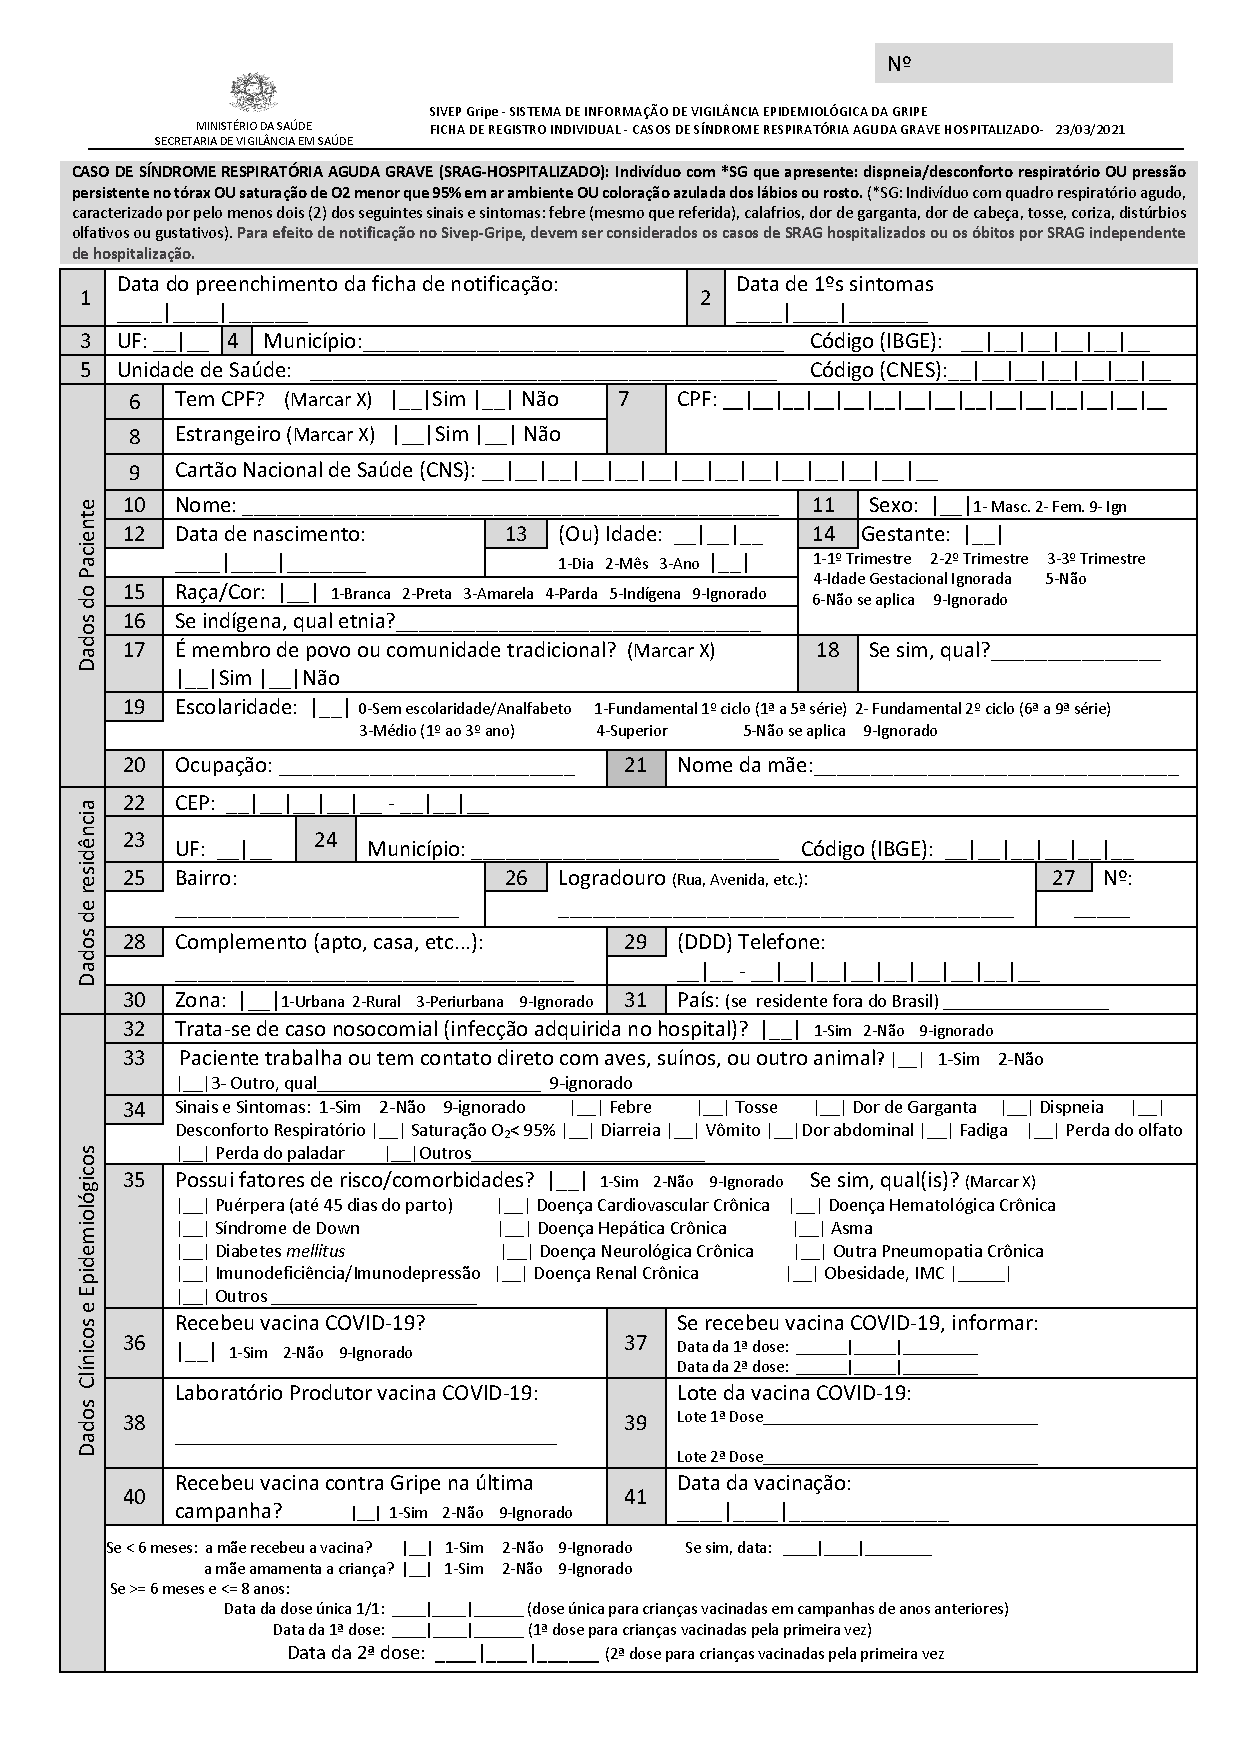
\includepdf[pages=-]{annex/ficha_srag_hospitalizado_23.03.2021.pdf}


    \chapter{Dicionário de dados}
    \label{ch:dicionario-de-dados}

    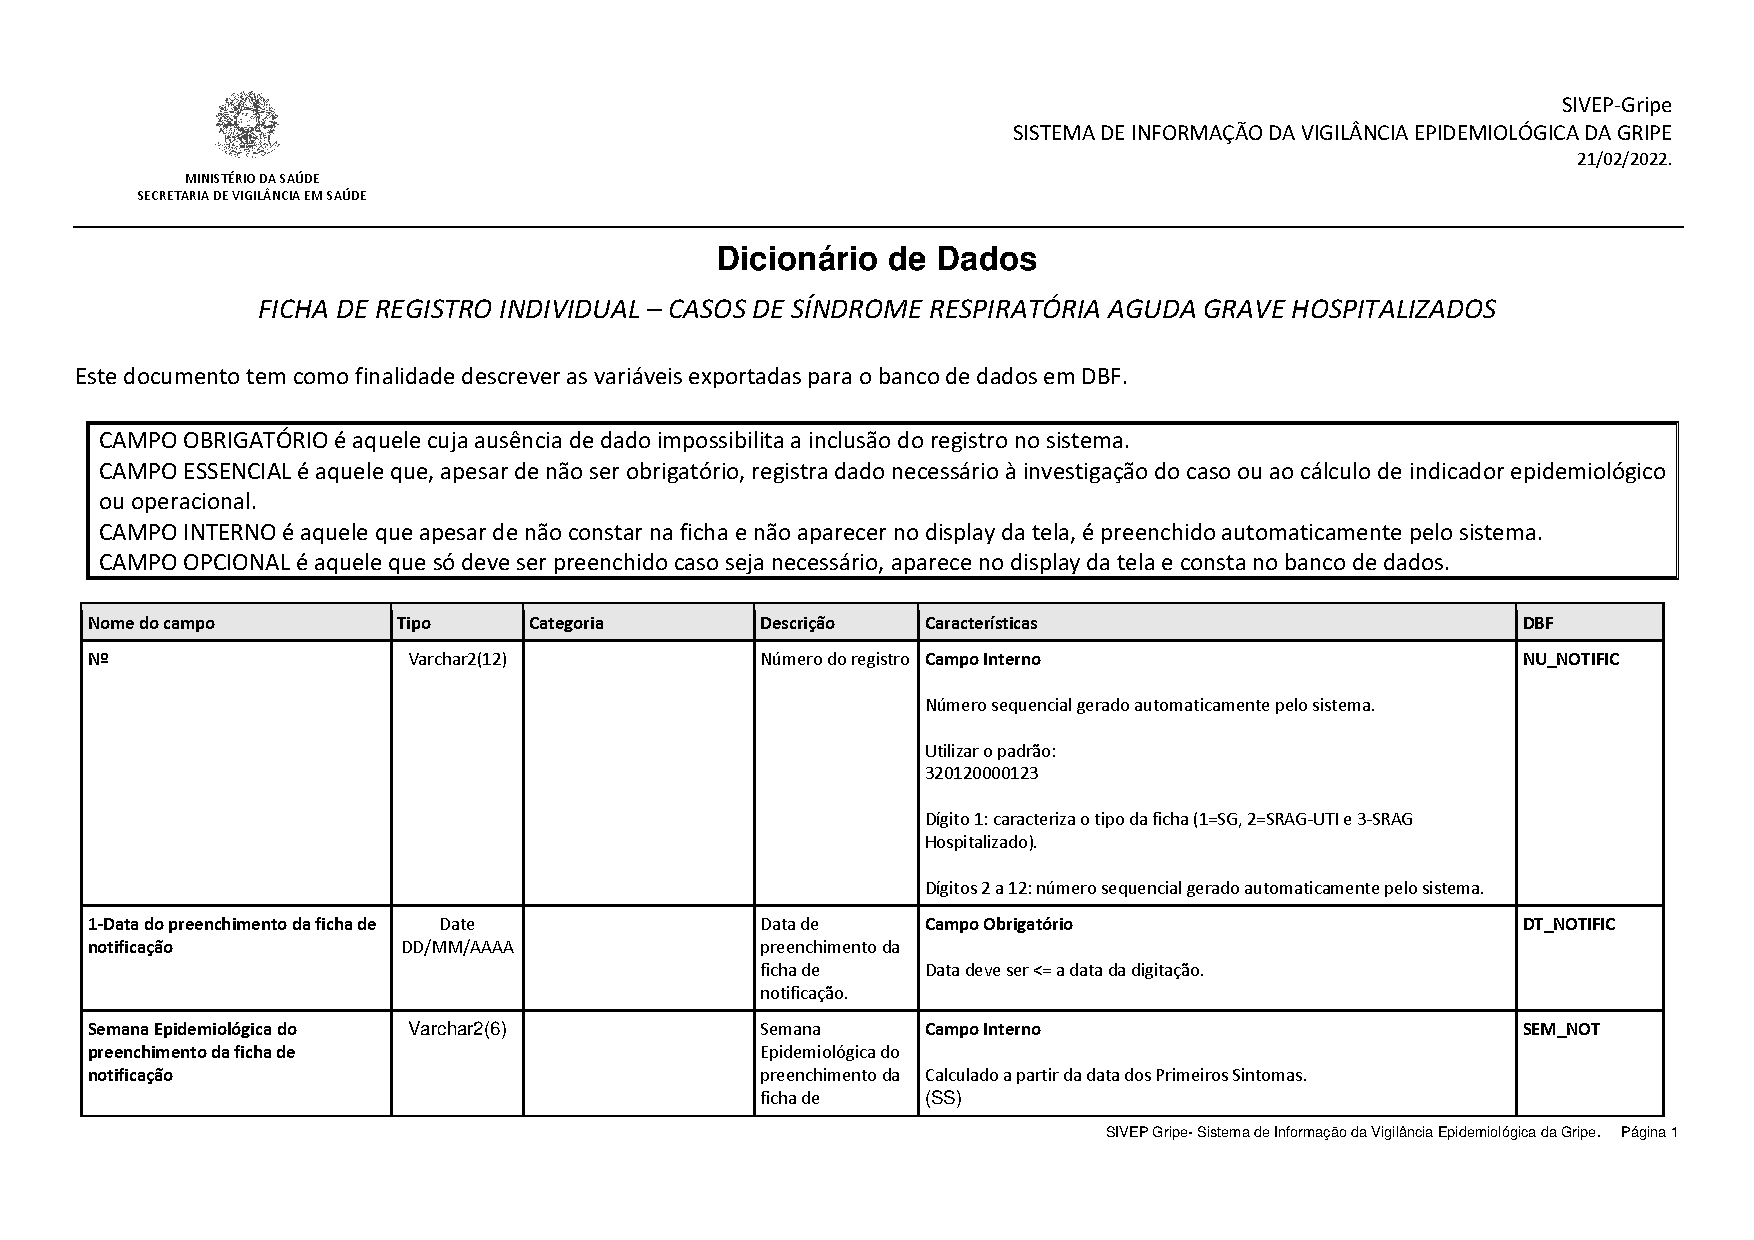
\includepdf[pages=-]{annex/dicionario_de_dados_srag_hosp_17_02_2022.pdf}

%
% Finalização do documento. A partir desse comando qualquer coisa escrita será ignorada:
%

\end{document}
